
%----------------------------------------------------------------------------------------
%	Lecture 7
%----------------------------------------------------------------------------------------

\chapter{Linear and Quadratic Approximations}

\bigbreak
\section{Linear Approximation}

\begin{figure}[ht!]
	\centering
	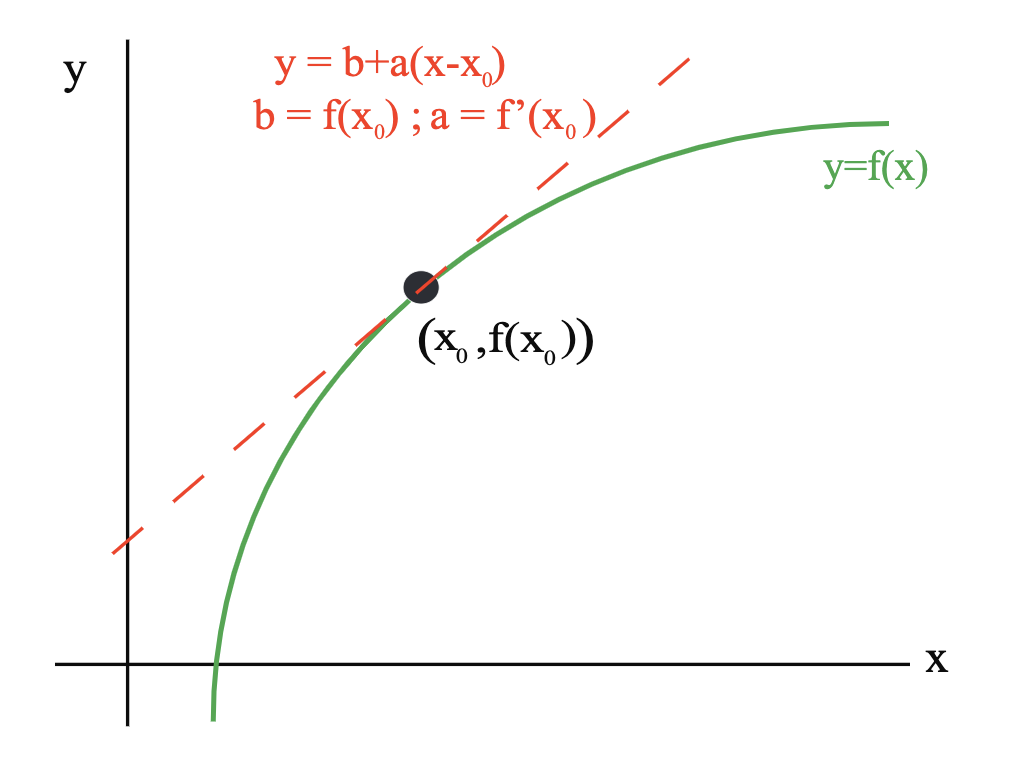
\includegraphics[scale=0.5]{./images/lecture_7_figure_1.png}
	\caption{Tangent as a linear approximation to a curve}
\end{figure}

The tangent line approximates $f(x)$. It gives good approximation near the point of tangency $x_0$.
As you move away from $x_0$, however, the approximation grows less accurate.
$$\boxed{ f(x) \approx f(x_0) + f'(x_0)(x-x_0) } $$

\subsection{Basic list of linear approximations}

In this list, we always use base point $x_0 = 0$ and assume $|x|<<1$.
\begin{enumerate}
	\item $\sin x	\approx x$ (If $x \approx 0$)
	\item $\cos x	\approx 1$ (If $x \approx 0$)
	\item $e ^ x	\approx 1 + x$ (If $x \approx 0$)
	\item $\ln(1+x)	\approx x$ (If $x \approx 0$)
	\item $(1+x)^r	\approx 1+rx$
\end{enumerate}

\section{Quadratic Approximation}

These are more complicated. They are only used when higher accuracy is needed.
$$ \boxed{
	f(x) \approx f(x_0) + f'(x_0)(x-x_0) + \frac{f''(x_0)}{2}(x-x_0)^2 \quad (x \approx x_0)
}$$

\subsection{Basic Quadratic Approximation}

\begin{enumerate}
	\item \ilds{ \sin x	\approx x } (If $x \approx 0$)
	\item \ilds{ \cos x	\approx 1 - \frac{x^2}{2} } (If $x \approx 0$)
	\item \ilds{ e ^ x	\approx 1 + x + \frac{x^2}{2} } (If $x \approx 0$)
	\item \ilds{ \ln(1+x)	\approx x - \frac{x^2}{2} } (If $x \approx 0$)
	\item \ilds{ (1+x)^r	\approx 1 + rx + \frac{r(r-1)}{2} x^2 } (If $x \approx 0$)
\end{enumerate}


\subsection*{Proofs}

Here, we will show the proofs for quadratic approximations.
For linear approximation, you can drop the quadratic term.

{\bf Proof of 1} : Take $ f(x) = \sin x \Rightarrow f'(x) = \cos x \Rightarrow f''(x) = - \sin x $.
Now $f(0) = 0$, $f'(0) = 1$ and $f''(0) = 0$.
So, $ \sin x \approx 0 + 1 \cdot x + 0 \cdot x^2 = x $

{\bf Proof of 2} : Take $ f(x) = \cos x \Rightarrow f'(x) = -\sin x \Rightarrow f''(x) = - \cos x $.
Now $f(0) = 1$, $f'(0) = 0$ and $f''(0) = -1$.
So, \ilds{ \cos x \approx 1 + 0 \cdot x + \frac{-1}{2} \cdot x^2 = 1 - \frac{x^2}{2} }

{\bf Proof of 3} : Take $ f(x) = e^x \Rightarrow f'(x) = e^x \Rightarrow f''(x) = e^x $.
Now $f(0) = 1$, $f'(0) = 1$ and $f''(0) = 1$.
So, \ilds{ e^x \approx 1 + 1 \cdot x + \frac{1}{2} \cdot x^2 = 1 + x + \frac{x^2}{2} }

{\bf Proof of 4} : Take $ f(x) = \ln(1+x) \Rightarrow f'(x) = \frac{1}{1+x} \Rightarrow f''(x) = \frac{-1}{(1+x)^2} $.
Now $f(0) = 0$, $f'(0) = 1$ and $f''(0) = -1$.
So, \ilds{ \ln(1+x) \approx 0 + 1 \cdot x + \frac{-1}{2} \cdot x^2 = 1 + x - \frac{x^2}{2} }

{\bf Proof of 5} : Take $ f(x) = (1+x)^r \Rightarrow f'(x) = r(1+x)^{r-1} \Rightarrow f''(x) = r(r-1)(1+x)^{r-2} $.
Now $f(0) = 1$, $f'(0) = r$ and $f''(0) = r(r-1)$.
So, \ilds{ (1+x)^r \approx 1 + r \cdot x + \frac{r(r-1)}{2} \cdot x^2 = x }


